\newcommand{\myCoord}[1]{
  \tikz[remember picture]{\coordinate[remember picture] (#1) at (0,0);
    %\fill[red] (#1) circle[radius=1pt];
  }
}


\begin{tikzpicture}[remember picture]
  \tikzstyle{noMargin} = [inner sep=0mm, outer sep=0mm]
  \node[draw, noMargin, remember picture, anchor=north west,
  minimum width = 3cm,
  label={[label distance=-0.8cm,text depth=15pt,rotate=90]left:description}
  ](methodTech){
    \qquad
    \begin{tabular}{lll}
      \multicolumn{3}{l}{technology used for:}\\ 
      \multicolumn{2}{l}{\qquad detection}& \myCoord{mlInit}\\
      \multicolumn{2}{l}{\qquad segmentation}\\
      \multicolumn{2}{l}{\qquad post-processing}&\myCoord{mlFin}\\
      $\mathcal{S}$: & \multicolumn{2}{l}{Quick-Shift super-pixels}\\
      $\arg \min (U(\cdot))$:&\multicolumn{2}{l}{\acl{gc}}\\
      $D(\cdot)$:&\multicolumn{2}{l}{\tikz[noMargin, baseline=(img.north)]{\node[noMargin](img){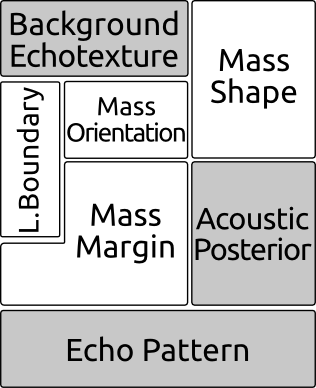
\includegraphics[width=1cm]{vcues}};}}\\
      &\multicolumn{2}{l}{\acs{rbf}-\acs{svm}}\\
      $V(\cdot,\cdot)$:&\multicolumn{2}{l}{Homogenity}\\
    \end{tabular}
  };
  \node[yshift=2pt,remember picture, overlay, nodeBase, mlStyle, fit= (mlInit) (mlFin)]{};
\node[draw, below= 2pt of methodTech,
minimum width = 3.9cm,
  label={[label distance=-0.5cm,text depth=15pt,anchor=south, rotate=90]left:testing}
  ](testingNode){
    \begin{tabular}{lclclc}
      \multicolumn{2}{l}{Database size:} & \multicolumn{4}{l}{$16$} \\
      \multicolumn{2}{l}{\ac{gt}:}       & \multicolumn{4}{l}{multi-label} \\
      \multicolumn{2}{l}{Task:}          & \multicolumn{4}{l}{$\mathcal{L} = \{\text{lesion}, \overline{\text{lesion}}\}$} \\
      \multicolumn{2}{l}{Trainning:}     & \multicolumn{4}{l}{Leave-one-Patient-Out}\\
      \ac{aov}:      & .623                                                                               & \ac{fpr}: & .4 & \ac{fnr}: & .008
    \end{tabular}
    };
%  \node[
%        draw=red,
%        minimum width=\textwidth,
%        fit=(current bounding box.north west) (current bounding box.south east),
%      ]at (current bounding box.center){};
\end{tikzpicture}

